 \subsection{Over-approximating the reach set of the nonlinear system}
\label{sec:x reach}

At time $k$, we need to compute the forward reach set, starting from $x_k$, for the next $N$ steps, for two purposes:
first, this is needed for defining the constraints on the input $v$ to the linearized dynamics.
Secondly, this is needed to compute a containing set for the estimation error in $z$-space.

In all but the simplest systems, forward reachable sets can not be computed exactly.
Moreover, the true state $x_k$ is not known.
Therefore we show how to compute an outer-approximation $\oaXset{k+j}{k},  j=0,\ldots, N$.
To do so we may use a reachability tool for nonlinear systems, RTreach??. 
A reachability tool computes an outer-approximation of the reachable set of a system starting from some set $\Xc \subset X$, subjet to inputs from a set $U$, for a duration $T \geq 0$. 
Denote this approximation by $\RT{\Xc}$.

At time $k$, the state estimate $\hx_{k}$ is known.
Therefore $x_k = \hx_{k} - e_k \in \hx_{k} \oplus (-E) \defeq \Xset{k}{k}$.
Propagating $\Xset{k}{k}$ forward one step through the continuous-time nonlinear dynamics yields $\Xset{k+1}{k}$, which is outer-approximated by $\RT{\Xset{k}{k}}$.
The estimate that the system will receive at time $k+1$ is therefore bound to be in the set $\RT{\Xset{k}{k}}  \oplus E$.
Since $0 \in E$, we maintain $\Xset{k+1}{k} \subset \RT{\Xset{k}{k}}  \oplus E$.
We define the over-approximate reach set at $k+1$, computed at time $k$, to be 
\begin{equation*}
\label{eq:def Xk}
\oaXset{k+1}{k} \defeq  \RT{\Xset{k}{k}}  \oplus E \oplus  (-E)
\end{equation*}
%(The reason for adding the extra $-E$ term will be apparent in the proof to Thm.??).
Fig. \ref{fig:overreach_NL} shows a visualization of this approach.

More generally, for $1 \leq j \leq N$, we define the $j$-step reach set computed at time $k$ to be
\begin{eqnarray}
\label{eq:def Xkj}
\oaXset{k}{k} &\defeq&   \hx_{k} \oplus (-E) 
\nonumber
\\
\oaXset{k+j}{k} & \defeq& \RT{\oaXset{k+j-1}{k}} \oplus E \oplus (-E) 
\end{eqnarray}

The following holds by construction:
\begin{lemma}
	\label{lemma:xreach}
	For any time $k$ and step $j \geq 1$, the $j$-step reach set of the non-linear dynamics starting from $x_k$ is outer-approximated by $\oaXset{k+j}{k}$:
	$\Xset{k+j}{k} \subset \oaXset{k+j}{k}$.
\end{lemma}


\begin{figure*}
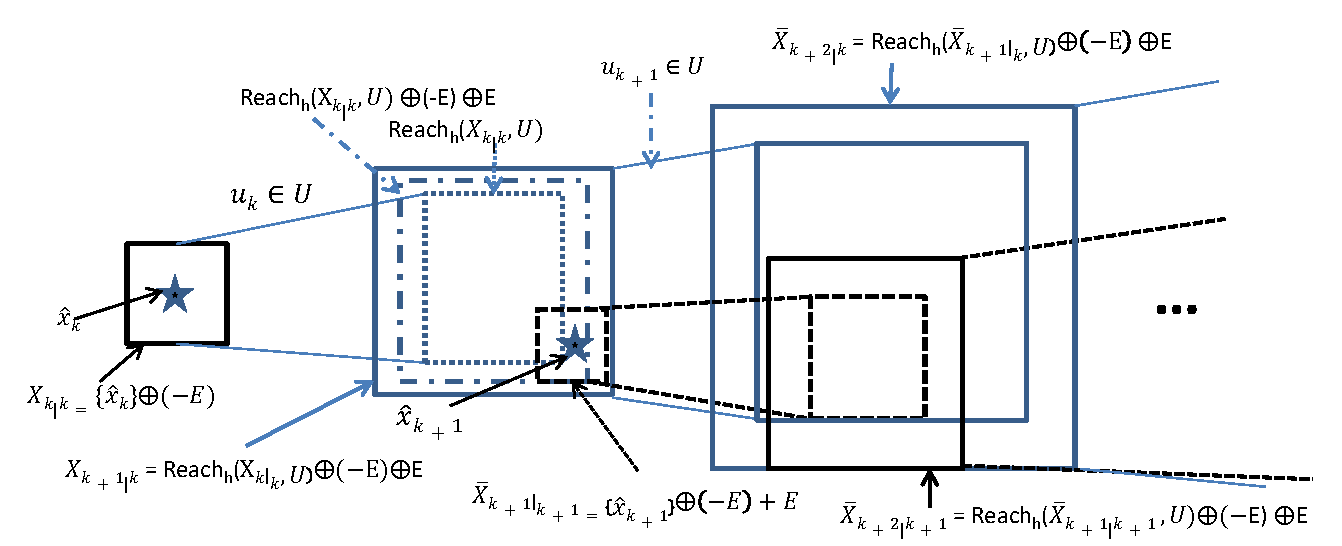
\includegraphics[scale=0.75]{figs/OverReachFigure_NL_scissored.pdf}
\caption{The over-approximated reachable sets for $x_{k+j}$, computed at time steps $k$, and correspondingly ay $k+1$ , used to compute $\tilde{E}_{k+j|k}$, $\underline{V}_{k+j|k}$. }
\label{fig:overreach_NL}
\end{figure*}

This construction of the outer-approximation permits us to prove recursive feasibility of the MPC controller,  because it causes the constraints of the MPC problem setup at time $k+1$ to be consistent with (stronger than) the constraints of the MPC problem setup at time $k$.
This will be explicitly stated and proved in the proof of Thm. ??